\documentclass[..\EOYR.tex]{subfiles}

\begin{document}

\section{The Dynamics of the Gulf Stream}
\label{SEC:DynamicsGulfStream}

The Gulf stream separates at Cape Hatteras, skirts the Grand Banks at Newfoundland and then heads Eastwards towards western Europe. However, in many moderate resolution climate models this separation occurs further north than observed and turns more sharply to the East, as noted in \citep{Hurlburt2008} and often misses off the Grand Banks, heading straight towards Europe. This can lead to what modellers refer to as the "blue spot of death" \citep{Gnanadesikan2007}, a patch of colder than observed SSTs resulting from the lack of heat at Newfoundland normally brought up by the Gulf Stream.

The exact cause for the path of the Gulf Stream is unknown, though it has been a research topic for many years and is still a popular topic amongst researchers today. A recurring theme when looking into the separation of the Gulf Stream is the mention of bathymetry. It is thought \citep{Gula2014}\citep{NaveiraGarabato2013}\citep{Nikurashin2012a} that the ocean dynamics resulting from the interaction of the Gulf Stream and the deep western boundary current (DWBC) with the bathymetry in the North Atlantic could cause the turbulence required to direct the Gulf Stream along its path. A sudden change in the direction of the Gulf Stream just off the coast at South Carolina and Georgia has been attributed by \citep{Gula2014} to the Charleston Bump, a topographical feature which raises the ocean floor, from a depth of 600m on the surrounding Blake Plateua to 200m. Hence it is clear that bathymetry can strongly impact the direction of ocean currents.


%\subsection{Subpolar Gyre \& subtropical gyre?}

\subsection{The Effects of topography}
\label{SSEC:EffectsOfTopography}

Ocean dynamics can be explained as a balance between the wind stress causing acceleration on the surface against the deceleration of the pressure forces resulting from the bathymetry \citep{NaveiraGarabato2013}.
%\citep{NaveiraGarabato2013} explain the dynamics of the ocean as a balance between the wind stress causing acceleration on the surface against the deceleration of the pressure forces resulting from the bathymetry.
The extent of the impact of topography on ocean dynamics can be seen by examining the difference between flat bottom models and models with realistic bathymetry.
%\td{Introduce the equations here with bpt and jebar? one of the papers does a really good job of justifying this - maybe greatbatch or gula? include some of the Gula or Yeager figures}

There are many ways to look into these differences, but we will focus mainly on two terms, the bottom pressure torque and the Joint Effect of Baroclinicity And Relief (JEBAR), as used by \citep{Greatbatch1991}, \citep{Bell1999}, \citep{Gula2014} as well as many others. 


\subsubsection{The Joint Effect of Baroclinicity and Relief (JEBAR)}
\label{SSSEC:JEBAR}

The JEBAR term was first introducted to account for the effects of topography and baroclinicity after the unrealistic results yielded from the more traditional flat-bottomed models. \citep{Meyers1996} states that this term is crucial for accurate Gulf Stream separation.
The term arises from the barotropic vorticity equation after taking the curl of the vertically averaged zonal and meridional flow.
\par
We will follow the derivation of the JEBAR and bottom pressure torque terms used in \citep{Greatbatch1991} as it reveals the barotropic vorticity equation as a combination of a JEBAR term and a wind term, demonstrating the balance referenced by \citep{NaveiraGarabato2013}
%\todo{maybe cite someone else? GV?}.

First we introduce the horizontal momentum equations (\ref{EQN:MomU}) \& (\ref{EQN:MomV}), the hydrostatic relation (\ref{EQN:Hydrostatic}) and the continuity equation (\ref{EQN:Continuity}) determining flow in spherical coordinates

\input{Equations/MomU.tex}
\begin{equation}
    fu=-\frac{1}{a\rho_0}\frac{\partial p}{\partial \phi} + \frac{1}{\rho_0}\frac{\partial\tau_{z\phi}}{\partial z}
\label{EQN:MomV}
\end{equation}

\begin{equation}
    0=-\frac{\partial p}{\partial z} - \rho_0 b
\label{EQN:Hydrostatic}
\end{equation}

\begin{equation}
    \frac{1}{a\cos\phi}\left(\frac{\partial u}{\partial\lambda} + \frac{\partial}{\partial\phi}\left(v\cos\phi\right)\right) + \frac{\partial w}{\partial z}=0
\label{EQN:Continuity}
\end{equation}


taking the coordinates with $\lambda$ as the longitude, $\phi$ as the latitude and $z$ as the altitude from the sea surface $\left(z=0\right)$ upwards.
The remaining terms are: $u$, $v$, and $w$ are the zonal, meridional and vertical velocity; $a$ is the Earth's radius; $\rho_0$ is the density of seawater; $p$ is the pressure perturbation; $b=g\frac{\left(\rho-\rho_r\right)}{\rho_0}$ is the negative buoyancy (where $\rho_r=\rho_r(z)$, the horizontally averaged denisty at depth $z$, and $g$ is the acceleration due to gravity); and $\tau_{z\lambda}$ and $\tau_{z\phi}$ are turbulent Reynolds stresses.\\
In line with the \citep{Greatbatch1991} derivation 
%and \td{citep{Mellor TODO}}
we neglect the local time derivative, nonlinear advection and horizontal Reynolds stress as we are focused on the vertical integration of the equations.
%\todo{See paper for explanation or not?}


First we introduce the notation
\begin{equation}
    U=\int_{-H}^0 u \, \text{d}z,\quad V=\int_{-H}^0 v \, \text{d}z.
\label{EQN:UVInt}
\end{equation}

We now establish a streamfunction $\psi$ satisfied by $U$ and $V$ by taking the vertical integral of (\ref{EQN:Continuity})
\begin{equation}
    \frac{1}{a\cos\phi}\left(\frac{\partial U}{\partial\lambda} + \frac{\partial}{\partial\phi}\left(V\cos\phi\right)\right)=0.
\label{EQN:VIntContinuity}
\end{equation}

We then have the define the required streamfunction by
\begin{equation}
    aU=-\frac{\partial\psi}{\partial\phi}\,,\quad aV\cos\phi=\frac{\partial\psi}{\partial\lambda}.
\label{EQN:Streamfunction}
\end{equation}

%
Taking the vertical averages of (\ref{EQN:MomU}) and (\ref{EQN:MomV}) gives
\begin{equation}
    -\frac{fV}{H} = -\frac{1}{Ha\rho_0\cos\phi}\int_{-H}^0\frac{\partial p}{\partial\lambda} \, \text{d}z + \frac{1}{H\rho_0}\left[\tau_\lambda^s-\tau_\lambda^b\right]
\label{EQN:VAvU}
\end{equation}


\begin{equation}
    \frac{fU}{H} = -\frac{1}{Ha\rho_0}\int_{-H}^0\frac{\partial p}{\partial\phi} \, \text{d}z + \frac{1}{H\rho_0}\left[\tau_\phi^s-\tau_\phi^b\right]
\label{EQN:VAvV}
\end{equation}

where $\left(\tau_\lambda^s, \tau_\phi^s\right)$ and $\left(\tau_\lambda^b, \tau_\phi^b\right)$ are the surface wind stresses and bottom stresses respectively. Following \citep{Greatbatch1991} we take the bottom stress to be zero $\left(\tau_\lambda^b=\tau_\phi^b=0\right)$.\\

Now we multiply through by $a$ and cross differentiating the vertically integrated momentum equations using

\begin{equation}
    \frac{\partial}{\partial \lambda}\left(\ref{EQN:VIntV}\right)-\frac{\partial}{\partial \phi}\left(\ref{EQN:VIntU}\right)\cos\phi
\label{EQN:CrossDifferential}
\end{equation}

and substituting for the streamfunction defined in (\ref{EQN:Streamfunction}) and the hydrostatic relation (\ref{EQN:Hydrostatic}) for the pressure terms, yields

\begin{equation}
\begin{split}
    \frac{\partial\psi}{\partial\phi}\frac{\partial}{\partial\lambda}\left(\frac{f}{H}\right) - \frac{\partial\psi}{\partial\lambda}\frac{\partial}{\partial\phi}\left(\frac{f}{H}\right) 
    = \frac{\partial}{\partial\phi}\frac{1}{H}\frac{\partial}{\partial\lambda}\left(\int_{-H}^0zb\, \text{d}z\right) - \frac{\partial}{\partial\lambda}\frac{1}{H}\frac{\partial}{\partial\phi}\left(\int_{-H}^0zb\, \text{d}z\right)  \\
    + \frac{a}{\rho_0}\left[\frac{\partial}{\partial\lambda}\left(\frac{\tau_\phi^s}{H}\right)-\frac{\partial}{\partial\phi}\left(\frac{\tau_\lambda^s\cos\phi}{H}\right)\right].
\end{split}
\label{EQN:FullCrossDifferential}
\end{equation}


By letting

\begin{equation}
    \Phi=\int_{-H}^0zb\,\text{d}z
\label{Phi}
\end{equation}

and using the Jacobian operator, we can separate (\ref{EQN:FullCrossDifferential}) into three terms

\begin{equation}
    J\left(\psi,\frac{f}{H}\right) = J\left(\Phi,\frac{1}{H}\right) + \frac{a}{\rho_0}\left[\frac{\partial}{\partial\lambda}\left(\frac{\tau_\phi^s}{H}\right)-\frac{\partial}{\partial\phi}\left(\frac{\tau_\lambda^s\cos\phi}{H}\right)\right]
\label{EQN:VorticityBalance}
\end{equation}

resulting in the desired form. The term on the left hand side of the eqaution represents the transport across $f/H$ contours, which is driven by the two terms on the right hand side. The first term on the right hand side of the equation is the JEBAR term and the second is the vorticity input from the wind.

This representation of the streamfunction driven by two separate forces has lead researchers to split the streamfunction into separate parts to allow further investigation. \citep{Greatbatch1991} follow on from their derivation of the above terms to later separate $\psi$ into three parts, one driven by the wind terms and two parts driven by the differnt aspects of the JEBAR term. 
%\todo{Add We'll explore this in a minute?} \todo{rewrite this}


%\td{Then discuss interpretation below - maybe show some figures from other papers}


%TODOThis term vanishes in the presence of smooth bathymetry \td{show this}

%TODOSplitting the JEBAR term:



\subsubsection{Bottom Pressure Torque}
\label{SSSEC:BPT}

%TODO\td{Intro about bottom pressure torque as for JEBAR}
We arrive at the bottom pressure torque in similar way to JEBAR, however instead of taking the curl of the vertically averaged flow, we now take the curl of the vertically integrated zonal and meridional flow.
Again we follow the derivation of \citep{Greatbatch1991}.

Vertically integrate the momentum equations (\ref{EQN:MomU}) and (\ref{EQN:MomV}) over the depth of the water column to obtain HERE
\begin{equation}
-fV = -\frac{1}{a\rho_0\cos\phi}\left[\frac{\partial}{\partial \lambda}\left(\int_{-H}^0p\,\text{d}z\right)-p_b H_\lambda\right]+\frac{1}{\rho_0}\left(\tau_\lambda^s-\tau_\lambda^b\right)
\label{EQN:VIntU}
\end{equation}

\begin{equation}
    fU = -\frac{1}{a\rho_0}\left[\frac{\partial}{\partial \phi}\left(\int_{-H}^0p\,\text{d}z\right)-p_b H_\phi\right]+\frac{1}{\rho_0}\left(\tau_\phi^s-\tau_\phi^b\right)
\label{EQN:VIntV}
\end{equation}

where $p_b$ is the bottom pressure and we take $\tau_\lambda^b=\tau_\phi^b=0$ as before.\\
Multiplying through by $a$, cross differentiating (taking the curl) of (\ref{EQN:VIntU}) and (\ref{EQN:VIntV}) as in (\ref{EQN:CrossDifferential}), using (\ref{EQN:VIntContinuity}) and substituting for the streamfunction defined in (\ref{EQN:Streamfunction}), yields

\begin{equation}
    \left(\frac{\text{d}f}{\text{d}\phi}\right)\frac{\partial \psi}{\partial\lambda} = \frac{1}{\rho_0}\left(-\frac{\partial p_b}{\partial\phi}\frac{\partial H}{\partial\lambda} + \frac{\partial p_b}{\partial\lambda}\frac{\partial H}{\partial\phi}\right)
    + \frac{a}{\rho_0}\left[\frac{\partial}{\partial\lambda}\left(\tau_\phi^s\right)-\frac{\partial}{\partial\phi}\left(\tau_\lambda^s\cos\phi\right)\right].
\label{EQN:CrossDifferentialVInt}
\end{equation}

%\todo{Understand the terms}

The first term on the right hand side of this equation corresponds to the bottom pressure torque and can be represented using the Jacobian as

\begin{equation}
    J(p_b,H) = - \frac{\partial p_b}{\partial \phi}\frac{\partial H}{\partial\lambda} + \frac{\partial p_b}{\partial\lambda}\frac{\partial H}{\partial \phi}.
\label{EQN:BPT}
\end{equation}


The second term on the right hand side of (\ref{EQN:CrossDifferentialVInt}) is the surface wind stress.

\citep{Greatbatch1991} show that if the bottom pressure torque in term in (\ref{EQN:CrossDifferentialVInt}) is 0, we are left with the flat-bottomed Sverdrup relation. Thus the bottom pressure torque term accounts for the effects of the bottom topography on the flow. \citep{Greatbatch1991} go on to separate the the streamfunction into two parts, one driven by the bottom pressure torque and the other driven by the flat-bottomed Sverdrup relation.
\par The impact of the bottom topography is demonstrated well by examining Figure \ref{FIG:Greatbatch1991Fig1Fig5Fig6}, comparing three figures from \citep{Greatbatch1991}. \ref{FIG:Greatbatch1991Fig1Fig5Fig6} shows the total streamfunction in a) and then decomposed into the case of no topography, driven only by the flat-bottomed Sverdrup relation in b), and the contribution from the bottom pressure torque term in c). It is evident that although the result is a combination of the terms, there is a significant impact on the transport by the twisting forces resulting from the bottom pressure torque, especially in areas key for the Gulf Stream (such as the area around the Grand Banks).

\begin{figure}[t]
    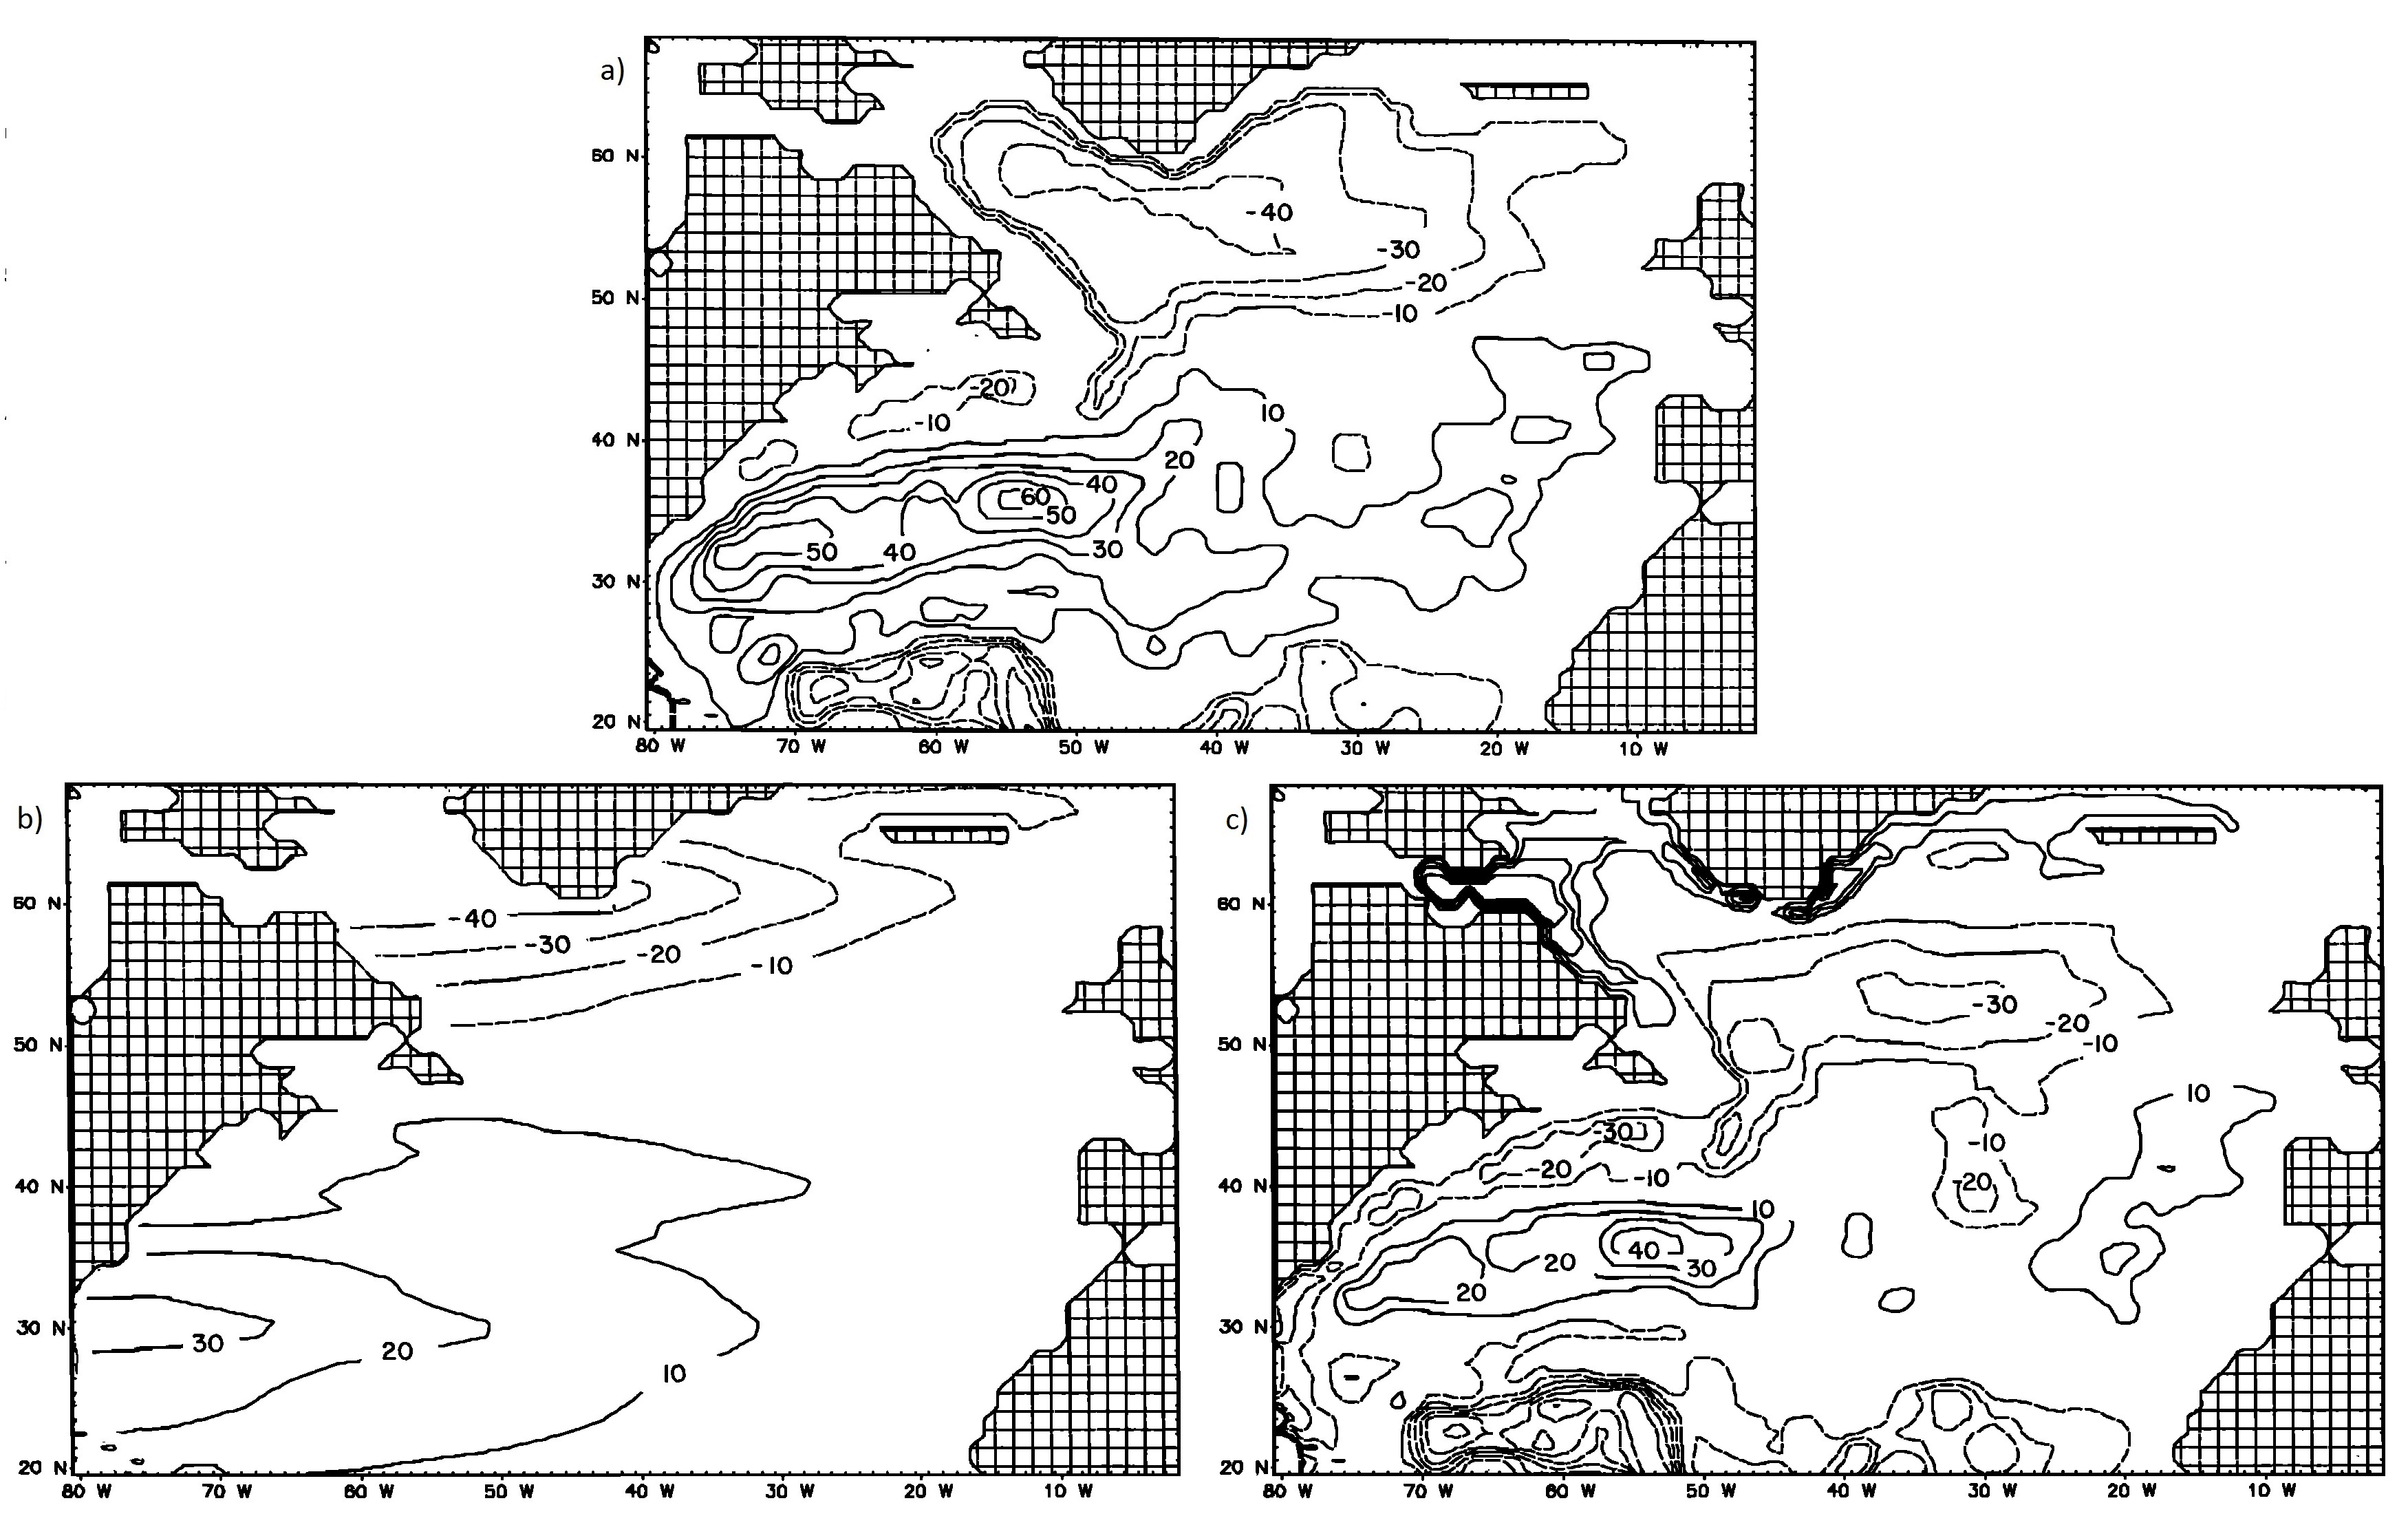
\includegraphics[width=\linewidth]{Figures/Greatbatch1991Fig1Fig5Fig6.jpg}
    \caption{a) The Transport stream function (annual mean field) calculated using climatological mean wind density data. The contour interval is 10Sv. Dashed contours indicate negative values; solid contours, positive values. b) As a) but for a flat-bottomed ocean. c) As a) but showing only the contributions from the bottom pressure torque (Figs. 1, 5 and 6 from \citep{Greatbatch1991})}
    \label{FIG:Greatbatch1991Fig1Fig5Fig6}
\end{figure}



It has been shown that the effect of bottom pressure torque with the DWBC has a strong impact on the NRG and thus the dynamics affecting the Gulf Stream \citep{Zhang2007}. Thus when trying to understand the separation of the Gulf Stream it is important to consider the bottom pressure torque.
%The bottom pressure torque is important for the separation of the Gulf Stream, it has been shown that the effect of bottom pressure torque with the DWBC has a strong impact on the NRG and thus the dynamics affecting the Gulf Stream \citep{Zhang2007}.

%The bottom pressure torque is important for the separation of the Gulf Stream as \citep{Zhang2007} showed that the effect of bottom pressure torque with the DWBC has a strong impact on the NRG and thus the dynamics affecting the Gulf Stream.




%TODO link bottom presure torque and JEBAR - The two terms are linked but represent different effects of the topography.




%\subsubsection*{Bototm Vortex Stretching}

\subsection{Small Scale Processes}
\label{SSEC:SmallScaleProcesses}

It has been noted that in higher resolution models, the separation and subsequent path of the Gulf Stream is much more accurate than in the lower resolution counterparts \citep{Hurlburt2008}\citep{Zhang2007}. This lends to the idea that the processes which affect the Gulf Stream occur on smaller scales which aren't resolved by coarser models \citep{NaveiraGarabato2013}\citep{Nikurashin2012a}. Various processes have been investigated and suggested as the main influences though it is likely that the improved Gulf Stream representation is due to multiple factors.


\citep{NaveiraGarabato2013} theorised that interaction with the bathymetry creates small-scale turbulence and instabilities which could cause bathymetric steering and divert currents. If this is not being represented in coarser models, the energy behind the turbulence must be going elsewhere. \citep{Scott2010} compared current meter readings with modelled values for kinetic energy and noticed that in some areas of the North Atlantic the total kinetic energy was being held higher in models than observed. It is discrepancies such as this which could have much wider implications. If the energy is not penetrating to the ocean floor, we cannot expect to be able to replicate the effects of the bathymetry. Perhaps by pulling this energy further down (closer to observed values), there would be more energy transfer from the larger ocean eddies to the smaller scale turbulence resulting from interaction with the bathymetry.

\citep{Tansley2001} used a simplified model of water flowing past a cylinder to highlight the importance of turbulence on fluid motion. 
Using a quarter-cylinder (mimicking a simplified version of Cape Hatteras) and a high Reynolds number (allowing for more turbulent flow), the model produced a jet with surrounding turbulent eddies similar to those observed in the Gulf Stream
%, a comparison between the two can be seen in Figure \ref{FIG:Tansley2001Fig10b}
. These results were not seen with a lower Reynolds number, highlighting the importance of turbulence in forming jets like the Gulf Stream.

%\begin{figure}[t]
    %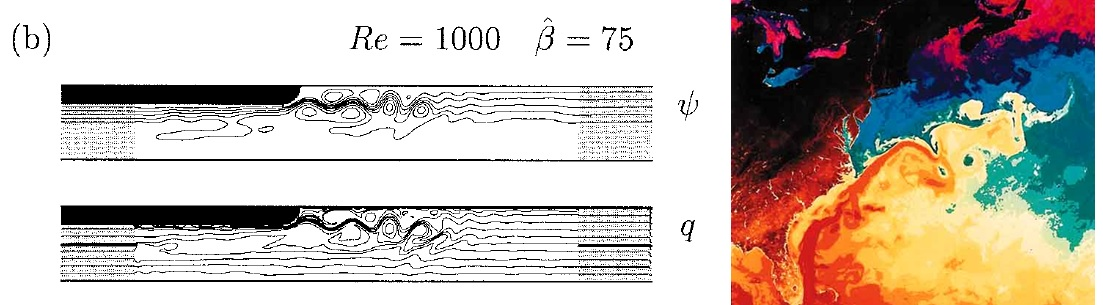
\includegraphics[width=\linewidth]{Figures/Tansley2001Fig10b.jpg}
    %\caption{Fig 10b) from \citep{Tansley2001} next to an image of the Gulf Stream, depicted by ocean temperatures in the North Atlantic (Reds warmest, blues and violets the coolest) from \citep{NASAHist}.}
    %\label{FIG:Tansley2001Fig10b}
%\end{figure}

The turbulent mixing arising from interaction with the bathymetry could allow geostrophic eddies to transfer some of their energy to smaller processes by causing internal waves to break and contribute to enhanced mixing \citep{Nikurashin2012a}. These effects have been seen even in cases of small-scale bathymetric roughness suggesting that it is not necessary to have large topological features to impact ocean dynamics, instead small surface differences can cause changes which lead to bigger outcomes.

\citep{NaveiraGarabato2013} attribute the significant impact of small-scale bathymetry to wave drag. Although wave drag is not a large contributor to ocean dynamics, topological features on a small scales can cause wave drag which contributes ten to several tens of a percentage of the dominant source and sink terms influencing the vorticity of the ocean.


These effects of small-scale processes are not limited to the Gulf Stream, but impact on many aspects of ocean dynamics as the various currents and features affect one another. 
\citep{Ezer2016b} speculated that amongst other things, the northern branches of the Northern Recirculation Gyre (NRG) would have to be resolved in order to produce an accurate Gulf Stream in a model. \citep{Zhang2007} determined that a significant contribution to the generation of the NRG is the bottom vortex stretching resulting from a downslope DWBC, which is in turn the result of the interaction with bathymetry as the DWBC crosses the path of the Gulf Stream. Hence, bathymetric impact can circle around to affect many aspects of ocean dynamics.


%\subsection{Energy Dissipation}


\end{document}
